\documentclass{article}

\usepackage[utf8]{inputenc}
\usepackage{datetime}
\usepackage{amsthm}
\usepackage{amsmath}
\usepackage{amssymb}
\usepackage{enumitem}
\usepackage[USenglish]{babel}
\usepackage{listings}
\usepackage{graphicx}
\graphicspath{ {images/} }
\usepackage{subcaption}
\usepackage{float}
\usepackage[makeroom]{cancel}
\usepackage{afterpage}
\usepackage{capt-of}
\usepackage{hyperref}

\DeclareMathOperator*{\argmin}{arg\,min}
\DeclareMathOperator*{\argmax}{arg\,max}

\title{ELE 538: Large-Scale Optimization \\ Final Report: ADMM in Neural Networks}
\author{Zachary Hervieux-Moore}

\newdate{date}{13}{05}{2018}
\date{\displaydate{date}}

\begin{document}

  \maketitle

  \clearpage

  \section{Introduction}

  In 2014, Goodfellow et al. introduced Generative Adversarial Networks (GANs) to the world \cite{goodfellow_2014}. GANs are able to synthetically create images that look realistic by cleverly using two neural networks. The first, called the generator, is fed a random noise vector and outputs an image. The second, called the discriminator, is fed images that it must classify as real or fake. By pitting these two networks against each other, the generator will become very good at creating images that resemble the real dataset. Since their seminal paper, many other applications of GANs have been created such as predicting the next frame in a video \cite{lotter_2015}, text to image generation \cite{reed_2016}, and creating a high resolution image from a low resolution one \cite{ledig_2016}. However, one problem in the training of GANs is the tendency of instability as the gradients find saddle points. This was the motivation of my final project; using ADMM during the optimization of neural networks to increase the stability of training. As a proof of concept, the first part of the project was to setup a toy problem was created using a neural network with ADMM used in the optimization. With this in hand, the second part was to setup a GAN and see the impacts of using ADMM in the optimization.

  \section{Background}

  To standardize the notation in the report, I will give a brief background of the material used during the final project. The first concept, that of the neural network, is rather simple. A neural network $f_\theta(\cdot)$ is simply a class of functions that are parameterized by $\theta$. In this case, the family of functions is a series of linear functions followed by a non linear function. We chose ReLU as our non linear function which is $\max(0,x)$. Note, this makes neural networks non convex. Here, $\theta$ represents the weights used in the linear functions. Then, finding the best neural network boils down to the standard statistics problem of

  \begin{gather*}
    \min_{\theta} \mathcal{L}(f_\theta(x), y)
  \end{gather*}
  where $\mathcal{L}(\cdot)$ is some loss function, $x$ are the inputs, and $y$ are the outputs.

  As mentioned earlier, a GAN is the combination of two neural networks that have competing loss functions which they are simultaneously trying to optimize. Formally, it is represented by the minimax problem

  \begin{gather*}
    \min_G \max_D = \mathbb{E}_{x \sim data} [\log D(x)] + \mathbb{E}_{z \sim p_z} [\log (1- D(G(z)))]
  \end{gather*}

  Where $D(x; \theta_d)$ is the discriminator network. It tries to minimize the error in the labels (real or generated). $G(z; \theta_g)$ is the generative network which takes in a noise vector $z$ and outputs something from your data space. Notice that the networks have their own independent sets of parameters. Here, the loss is cross entropy between the discriminator and real data as well as the discriminator and the output of the generator. Thus, the discriminator is trying to identify real and fake images correctly while the generator is trying to maximize the error in the discriminator.

  Finally, we come to ADMM which was taught in the class but presented here for completeness. ADMM are problems of the form
  \begin{gather*}
    \min f(x) + g(z) \\
    \text{s.t. } Ax + Bz = c
  \end{gather*}
  Which can be solved using the following iterations
  \begin{gather*}
    x^{k+1} = \arg\min_x L_\rho (x, z^k, \lambda^k) \\
    z^{k+1} = \arg\min_z L_\rho (x^{k+1}) \\
    \lambda^{k+1} = \lambda^k + \rho (A x^{k+1} + B z^{k+1} - c)
  \end{gather*}
  Here, $L_\rho(\cdot)$ is the augmented Lagrangian. These iterations can be significantly easier to compute. In the scope of the project, it hopefully improves the stability of neural network optimization by splitting the optimization into two parts.

  \section{Methods and Results}

  \subsection{Toy Problem}

  The first problem considered was a simple regression problem using a neural network. The data was drawn from a standard normal distribution, $x \sim \mathcal{N}(0, I)$ and the output was simply $y = AX + b$ where $A$ and $b$ were picked randomly. Thus, the data followed a linear model and the neural network was trained to try and retrieve this model. This was accomplished by using $L^2$ loss with a $L^2$ regularizer on the weights of the network:

  \begin{gather*}
    \min_\theta \lVert f_\theta (x) - y \rVert_2^2 + \frac{1}{2} \lVert \theta \rVert_2^2
  \end{gather*}

  Turning this optimization problem into ADMM, we split the two terms and put the constraint that the inputs into both terms must be equal

  \begin{gather*}
    \min_{\theta_1, \theta_2} \lVert f_{\theta_1} (x) - y\rVert_2^2 + \frac{1}{2} \lVert \theta_2 \rVert_2^2 \\
    \text{s.t. } \theta_1 = \theta_2
  \end{gather*}

  Calculating the ADMM iterations from this is straightforward and yields

  \begin{gather*}
    \theta_1^{k+1} = \arg\min_{\theta_1} \lVert f_{\theta_1}(x) - y \rVert_2^2 + \langle \lambda^k, \theta_2^k - \theta_1 \rangle + \frac{\rho}{2} \lVert \theta_2^k - \theta_1 \rVert_2^2 \\
    \theta_2^{k+1} = \frac{\theta_1^{k+1} - \lambda^k}{1 + \rho} \\
    \lambda^{k+1} = \lambda^k + \rho (\theta_2^{k+1} - \theta_1^{k+1})
  \end{gather*}

  A comparison was done of the loss value vs. iterations for both vanilla stochastic gradient descent optimization and optimization using the ADMM formulation. This is presented in Figure \ref{fig:toy-results}. The thing to note is that the optimization for the two were fairly similar. The ADMM was perhaps slightly faster but seemingly less stable. However, this may have been correctable with proper hyperparameter tuning which was not done to keep the other variables constant during the experiment. It is also interesting to note that the regularizer loss, $g$, increased overtime in the ADMM model but not the standard one. Finally, even though ADMM has seemingly more parts to the optimization, the wall clock time for one epoch of training was actually lower for ADMM.

  \begin{figure}[H]
    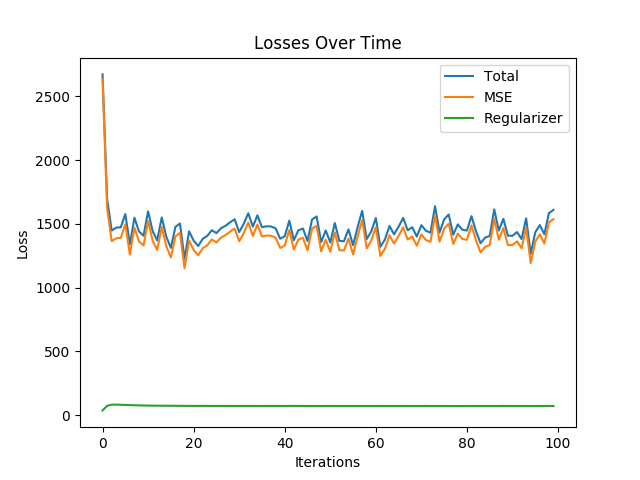
\includegraphics[width=0.4\linewidth]{./images/toy_loss.png}
    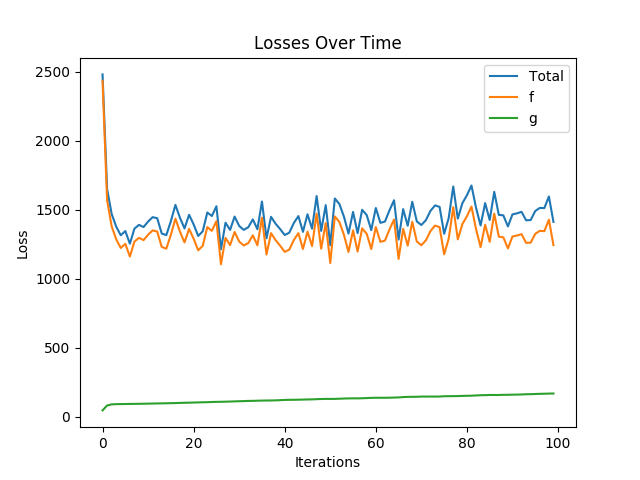
\includegraphics[width=0.4\linewidth]{./images/toy_admm_loss.png}
    \caption{Objective Value vs. Iterations for normal SGD on the left and ADMM on the right.}
    \label{fig:toy-results}
  \end{figure}

  \subsection{GANs}

  For the GAN experiment, we created used the DCGAN architecture. This is simply a GAN which utilized convolutions in the layers \cite{radford_2015}. Finally, the dataset of images used was MNIST. Using the minimax formulation of GANs from before, we get the following problem for the discriminator

  \begin{gather*}
    \min_{\theta_d} \log D(x; \theta_d) + \log (1 - D(G(z); \theta_d))
  \end{gather*}
  Following the steps of the toy problem, we formulate this as a ADMM problem
  \begin{gather*}
    \min_{\theta_{d_1}, \theta_{d_2}} \log D(x; \theta_{d_1}) + \log (1 - D(G(z); \theta_{d_2}))
  \end{gather*}
  Which yields the following iterations
  \begin{gather*}
    \theta_{d_1}^{k+1} = \arg\min_{\theta_{d_1}} \log D(x ; \theta_{d_1}) + \langle \lambda^k, \theta_{d_2}^k - \theta_{d_1} \rangle + \frac{\rho}{2} \lVert \theta_{d_2}^k - \theta_{d_1} \rVert_2^2 \\
    \theta_{d_2}^{k+1} = \arg\min_{\theta_{d_2}} \log(1 - D(G(z) ; \theta_{d_2})) + \langle \lambda^k, \theta_{d_2} - \theta_{d_1}^{k+1} \rangle + \frac{\rho}{2} \lVert \theta_{d_2} - \theta_{d_1}^{k+1} \rVert_2^2 \\
    \lambda^{k+1} = \lambda^k + \rho (\theta_{d_2}^{k+1} - \theta_{d_1}^{k+1})
  \end{gather*}

  Again, we saw faster training iteration times for the ADMM, but the results were not very good. This is due to the fact that the discriminator $d_1$ simply always outputs real and discriminator $d_2$ outputs fake. Figure \ref{fig:gan-normal} shows the generator outputs for the vanilla optimization and Figure \ref{fig:gan-admm} shows the generator outputs for ADMM optimization.

  \begin{figure}[H]
    \begin{center}
      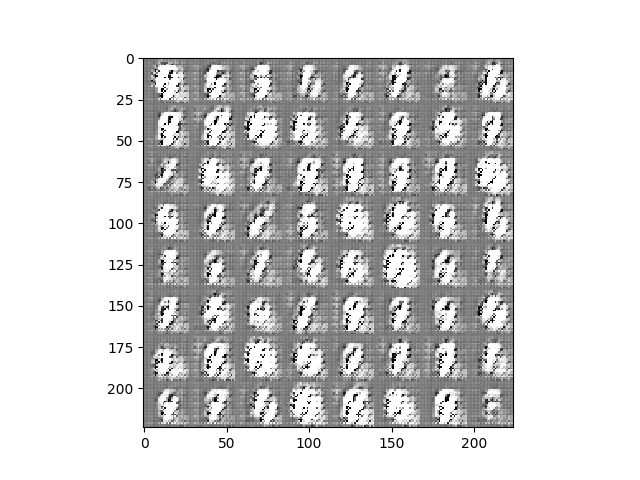
\includegraphics[width=0.2\linewidth]{./images/dcgan_50.png}
      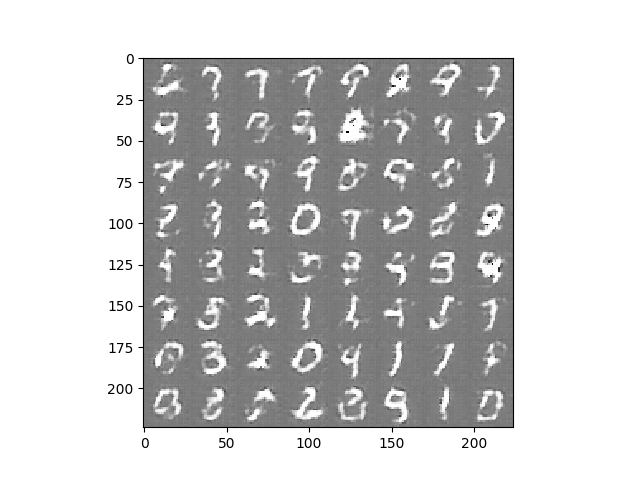
\includegraphics[width=0.2\linewidth]{./images/dcgan_150.png}
      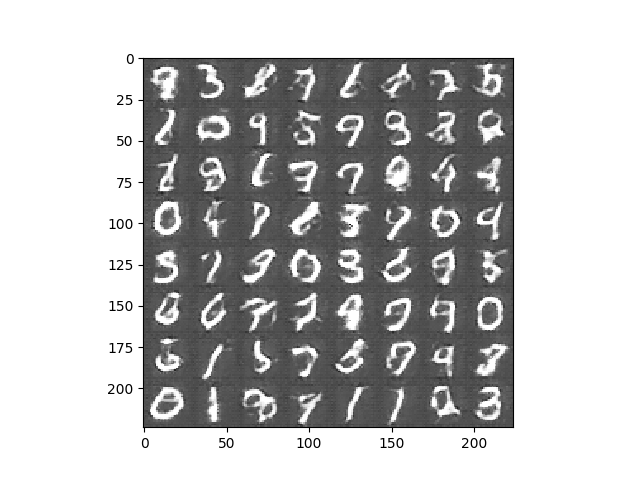
\includegraphics[width=0.2\linewidth]{./images/dcgan_250.png}
    \end{center}
    \caption{Generative examples from the non ADMM model at the 50, 150, and 250 epochs.}
    \label{fig:gan-normal}
  \end{figure}

  \begin{figure}[H]
    \begin{center}
      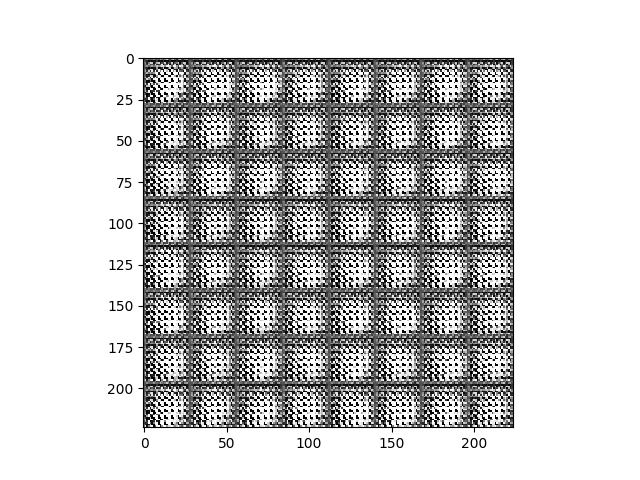
\includegraphics[width=0.2\linewidth]{./images/dcgan_admm_50.png}
      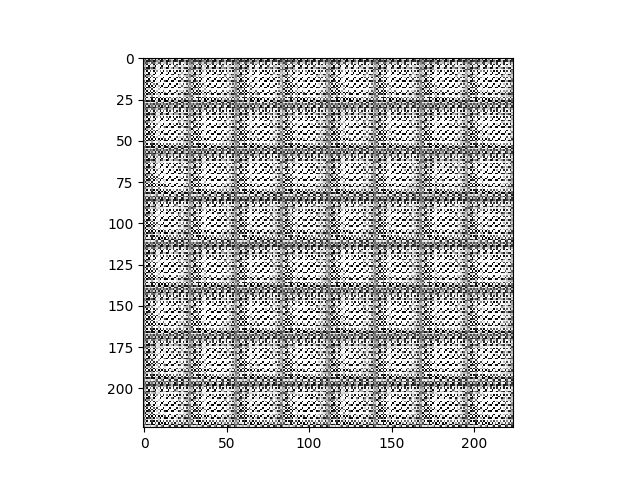
\includegraphics[width=0.2\linewidth]{./images/dcgan_admm_150.png}
      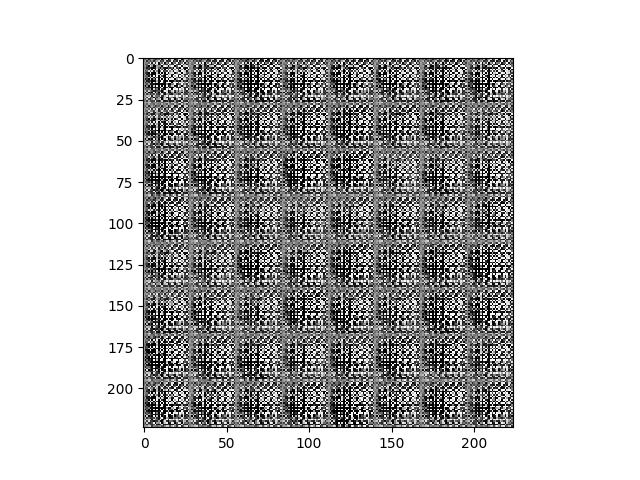
\includegraphics[width=0.2\linewidth]{./images/dcgan_admm_250.png}
    \end{center}
    \caption{Generative examples from the ADMM model at the 50, 150, and 250 epochs.}
    \label{fig:gan-admm}
  \end{figure}

  \section{Conclusion}

  While the result of using ADMM were not promising in training of GANs, it did work for the toy model and so does have some potential. It is also an interesting result that small pertubations in the parameter space of neural networks can yield networks that do the exact opposite of each other. For future directions, it would be interesting to see if enhancing the objective with another type of loss can prevent the degeneration of the ADMM training. Another avenue would be to interleave optimization steps using standard stochastic gradient descent and ADMM to see if performing ADMM sometimes as opposed to always would help with stability. The thought being that the weaknesses in both optimizations are cancelled out by performing a few iterations of the other.

  \clearpage

  \bibliography{references}
  \bibliographystyle{ieeetr}

\end{document}